\documentclass[aspectratio=169]{beamer}
\useoutertheme[progressbar=frametitle]{metropolis}
\useinnertheme{metropolis}


\definecolor{nabgray}{rgb}{0.6,0.59,0.61}
\usecolortheme[named=nabgray]{structure}

\usepackage{tikz}
\usepackage[utf8]{inputenc}
\usepackage[portuguese]{babel}

\usepackage{smartdiagram}
\usepackage{qtree}
\usepackage{verbatim}
\usepackage{svg}
\usepackage{graphicx}
\usepackage{color}

\definecolor{lightgray}{rgb}{0.95, 0.95, 0.95}
\definecolor{darkgray}{rgb}{0.4, 0.4, 0.4}
%\definecolor{purple}{rgb}{0.65, 0.12, 0.82}
\definecolor{editorGray}{rgb}{0.95, 0.95, 0.95}
\definecolor{editorOcher}{rgb}{1, 0.5, 0} % #FF7F00 -> rgb(239, 169, 0)
\definecolor{editorGreen}{rgb}{0, 0.5, 0} % #007C00 -> rgb(0, 124, 0)
\definecolor{orange}{rgb}{1,0.45,0.13}
\definecolor{olive}{rgb}{0.17,0.59,0.20}
\definecolor{brown}{rgb}{0.69,0.31,0.31}
\definecolor{purple}{rgb}{0.38,0.18,0.81}
\definecolor{lightblue}{rgb}{0.1,0.57,0.7}
\definecolor{lightred}{rgb}{1,0.4,0.5}
\usepackage{upquote}
\usepackage{listings}
\lstset{language=java,
	basicstyle=\footnotesize\ttfamily,
	keywordstyle=\footnotesize\color{blue}\ttfamily,
	escapeinside={<@}{@>}
}
\lstdefinelanguage{Kotlin}{
	comment=[l]{//},
	commentstyle={\color{gray}\ttfamily},
	emph={delegate, filter, first, firstOrNull, forEach, lazy, map, mapNotNull, println, return@},
	emphstyle={\color{purple}},
	identifierstyle=\color{black},
	keywords={abstract, actual, as, as?, break, by, class, companion, continue, data, do, dynamic, else, enum, expect, false, final, for, fun, get, if, import, in, interface, internal, is, null, object, override, package, private, public, return, set, super, suspend, this, throw, true, try, typealias, val, var, vararg, when, where, while},
	keywordstyle={\color{lightblue}\bfseries},
	morecomment=[s]{/*}{*/},
	morestring=[b]",
	morestring=[s]{"""*}{*"""},
	ndkeywords={@Inject, @Deprecated, @JvmField, @JvmName, @JvmOverloads, @JvmStatic, @JvmSynthetic, Array, Byte, Double, Float, Int, Integer, Iterable, Long, Runnable, Short, String},
	ndkeywordstyle={\color{orange}\bfseries},
	sensitive=true,
	stringstyle={\color{olive}\ttfamily},
}


\usebackgroundtemplate%
{%
	
\includegraphics[width=\paperwidth]{Images/Contenido.png}%
}


\title{O estado atual do Kotlin no backend}
\author{Víctor Orozco - Nabenik}
\institute{@tuxtor}
\date{\today}

\begin{document}
{
    \usebackgroundtemplate{
\includegraphics[width=\paperwidth]{Images/portada}}
    \setbeamercolor{frametitle}{fg=red}
    \usebeamercolor[fg]{normal text}
    \frame{\titlepage}
}


\begin{frame}[fragile]{Kotlin}
    \begin{columns}
        \begin{column}{0.5\textwidth}
            \begin{itemize}
                \item Linguagem (Kotlin)
                \item OpenJDK (Java Virtual Machine)
                \item Bibliotecas/API (Java Classpath)
                \item kotlin-stdlib
            \end{itemize}
        \end{column}
        \begin{column}{0.5\textwidth}  %%<--- here
            \begin{figure}
                \centering
                
\includegraphics[width=0.4\linewidth]{Images/kotlin}
            \end{figure}
        \end{column}
    \end{columns}
\end{frame}


{
    \usebackgroundtemplate{
\includegraphics[width=\paperwidth]{Images/separador}}
    \setbeamercolor{normal text}{fg=white}
    \setbeamercolor{frametitle}{fg=red}
    \usebeamercolor[fg]{normal text}
    \section{Paradigmas de desenvolvimento}
}



\begin{frame}[fragile]{Desenvolvimento na JVM}
    \begin{columns}
    
        \begin{column}{0.5\textwidth}
        Paradigma
            \begin{itemize}
                \item Thread 
                \item Async
            \end{itemize}
        \end{column}
        \begin{column}{0.5\textwidth}  %%<--- here
        Abragencia do toolkit
            \begin{itemize}
                \item DIY
                \item Micro
                \item Pilhas inclusas
            \end{itemize}
        \end{column}
    \end{columns}
\end{frame}


\begin{frame}[fragile]{Concorrência com threads}
Thread based -e.g. EJB, CDI, JAX-RS-. Uma conexão http = 1 thread
\begin{lstlisting}[language=Java]
@Inject
SayService say;

@GET
@Produces(MediaType.TEXT_PLAIN)
public String hello() {
    return say.hello();
}
\end{lstlisting}

JakartaEE/MicroProfile, Spring
\end{frame}


\begin{frame}[fragile]{Baseado em Async}
Reactive based -e.g. Async JAX-RS, Spring WebFlux, Actors, Verticles-
\begin{lstlisting}[language=Java]
public class Server extends AbstractVerticle {
  public void start() {
    vertx.createHttpServer().requestHandler(req -> {
      req.response()
        .putHeader("content-type", "text/plain")
        .end("Hello from Vert.x!");
    }).listen(8080);
  }
}
\end{lstlisting}
Vert.x, Spring WebFlux, Zio, Akka
\end{frame}


\begin{frame}{Arquitetura}

\begin{columns}
\begin{column}{0.5\textwidth}
\begin{itemize}
	\item Monólito
    \item Microserviço
    \item Micromonolito
\end{itemize}
\end{column}
\begin{column}{0.5\textwidth}  %%<--- here
\begin{figure}
	\centering
	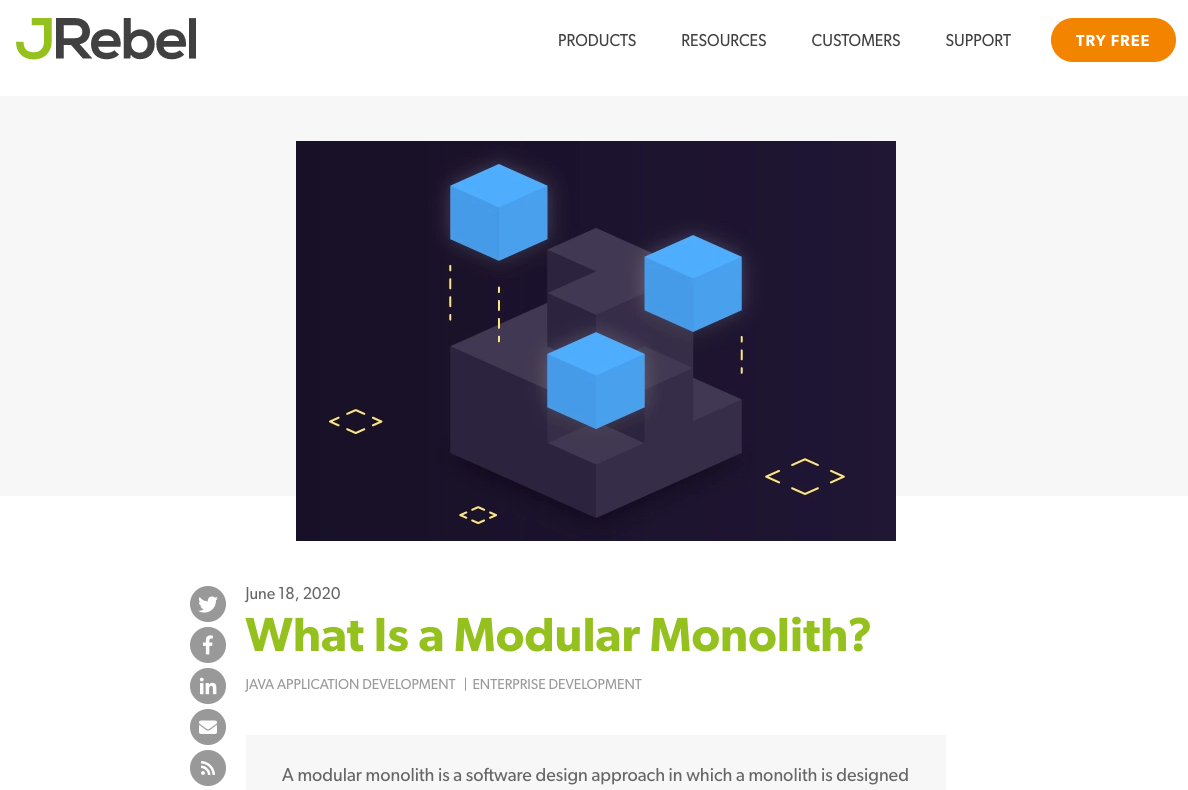
\includegraphics[width=0.9\linewidth]{Images/micromonolito.png}
\end{figure}
\end{column}
\end{columns}

\end{frame}


\begin{frame}{Runtime}

\begin{columns}
\begin{column}{0.5\textwidth}
"Simples/DIY"
\begin{itemize}
\item Servlet based -e.g. Tomcat, Jetty-
\item Custom I/O -e.g. Undertow, Netty, Vert.x-
\end{itemize}
\end{column}
\begin{column}{0.5\textwidth}  %%<--- here
\begin{figure}
	\centering
	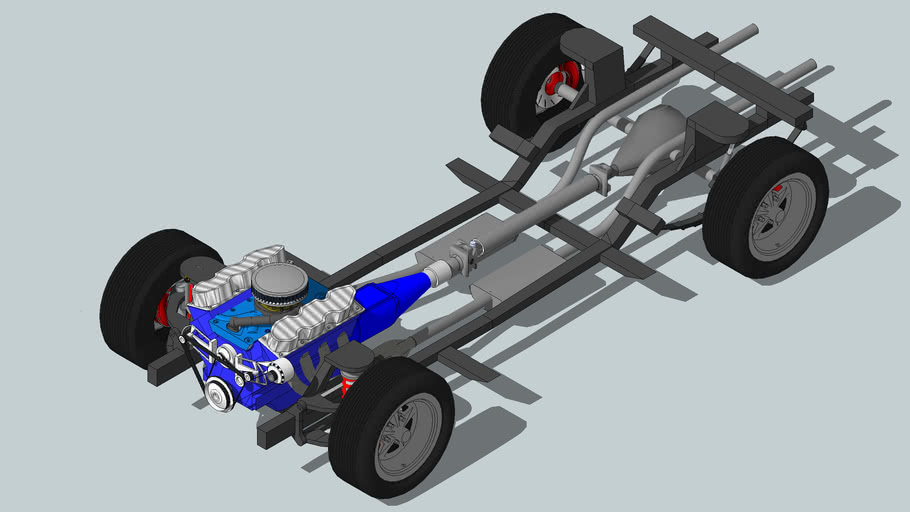
\includegraphics[width=0.9\linewidth]{Images/chassis}
\end{figure}
\end{column}
\end{columns}

\end{frame}


\begin{frame}{Runtime/Framework}

\begin{columns}
\begin{column}{0.5\textwidth}
"Micro"
\begin{itemize}
\item Custom micro -e.g. Jooby, Spark, Javalin, Helidon SE-
\item MicroProfile based -e.g. Quarkus, Helidon-
\item Micronaut
\item Spring Boot
\end{itemize}
\end{column}
\begin{column}{0.5\textwidth}  %%<--- here
\begin{figure}
	\centering
	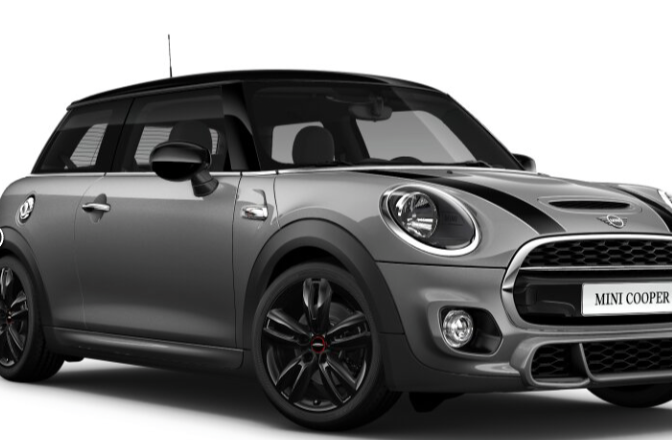
\includegraphics[width=0.9\linewidth]{Images/cooper}
\end{figure}
\end{column}
\end{columns}

\end{frame}

\begin{frame}{Complexo}

\begin{columns}
\begin{column}{0.5\textwidth}

"Complexo"
\begin{itemize}
\item Java EE/Jakarta EE -e.g. JBoss, WebSphere Liberty-
\item Spring
\item Akka
\end{itemize}
\end{column}
\begin{column}{0.5\textwidth}  %%<--- here
\begin{figure}
	\centering
	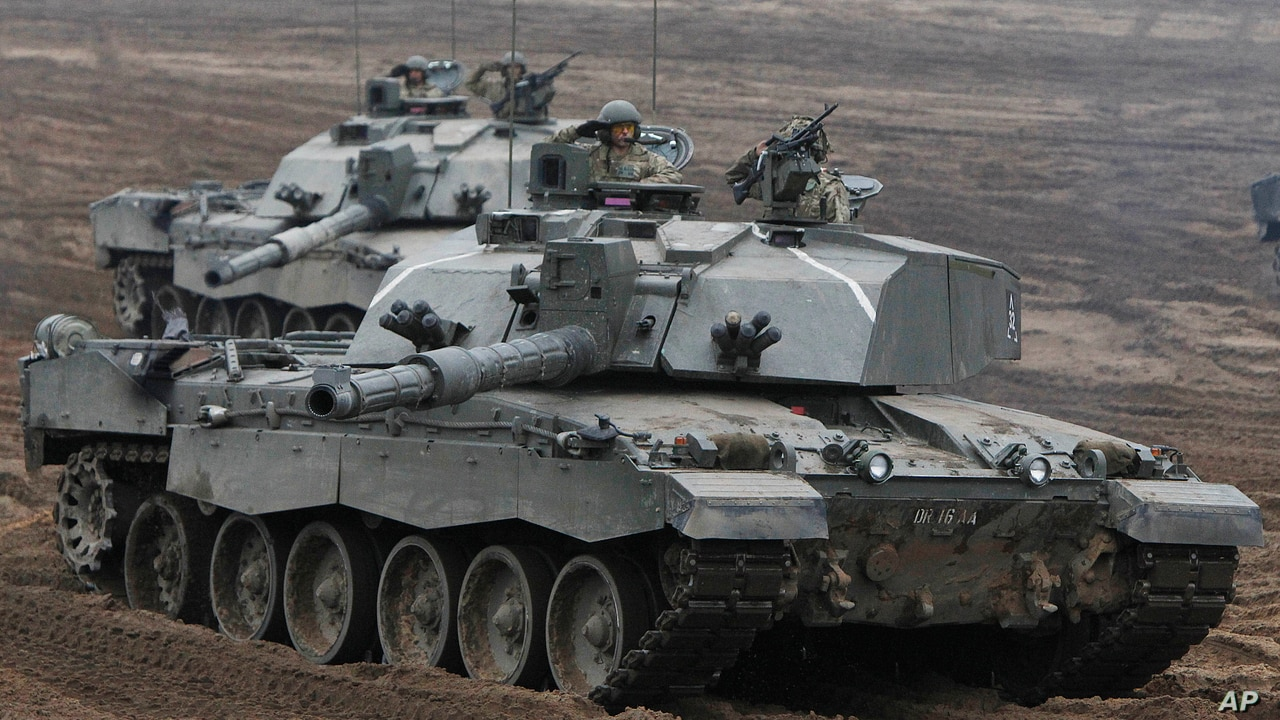
\includegraphics[width=0.9\linewidth]{Images/tank}
\end{figure}
\end{column}
\end{columns}

\end{frame}

\begin{frame}{Arquiteto no ano 2021}

\begin{exampleblock}{Arquiteto}
A pessoa que tem que decidir entre pegar um framework pronto \textit{complexo} ou pegar um runtime \textit{ligero} e criar a estrutura toda -i.e Bibliotecas, estilo arquitetural, SCM (Maven)-.\\


A pessoa que tem que decidir entre chatear os dev Java tradicionais no modelo de desenvolvimento Async ou chatear os desenvolvedores Kotlin por não aproveitar os Coroutines.\\

A pessoa que tem que avaliar o pulo para o Kotlin conservando (ou não) os stacks tradicionais.

\end{exampleblock}
\end{frame}

\begin{frame}{Arquiteto no ano 2021}

\begin{exampleblock}{Arquiteto}
A pessoa que vai ser odiada por não dar o pulo para JavaScript só pela vontade de re-escreber a base de código que vem fazendo sucesso há 15 anos
\end{exampleblock}
\end{frame}

{
    \usebackgroundtemplate{
\includegraphics[width=\paperwidth]{Images/separador}}
    \setbeamercolor{normal text}{fg=white}
    \setbeamercolor{frametitle}{fg=red}
    \usebeamercolor[fg]{normal text}
    \section{Kotlin no backend}
}


\begin{frame}{Kotlin no backend - Fatos}

\begin{exampleblock}{Fato \#1}
Todo framework Java pode virar framework Kotlin. Mas nem todo framework Java e testado no Kotlin.
\end{exampleblock}
\end{frame}

\begin{frame}{Kotlin no backend - Fatos}
\begin{figure}
	\centering
	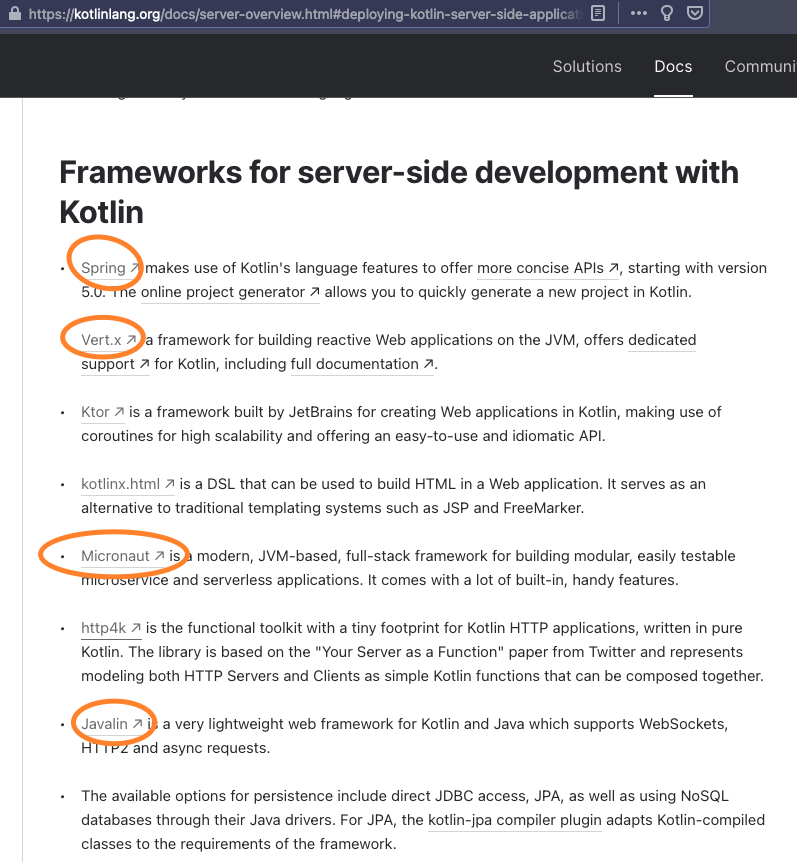
\includegraphics[width=0.55\linewidth]{Images/fwkotlin}
\end{figure}
\end{frame}

\begin{frame}{Kotlin no backend - Fatos}

\begin{exampleblock}{Fato \#2}
Geralmente o problema de não testar são os annotation processors -e.g. DeltaSpike-, muitos são feitos para o Java
\end{exampleblock}
\end{frame}

\begin{frame}{Kotlin no backend - Fatos}

\begin{exampleblock}{Fato \#3}
O ecosistema Kotlin esta criando Frameworks Kotlin-first/Kotlin-exclusive
\end{exampleblock}
\end{frame}

\begin{frame}[fragile]{Kotlin no backend - Fatos}
Reactive based - DIY
\begin{lstlisting}[language=Kotlin]
fun HelloWorld(): HttpHandler {
    return routes("/" bind GET to { Response(OK).body("hello world!") })
}
\end{lstlisting}
Http4k
\end{frame}

\begin{frame}[fragile]{Kotlin no backend - Fatos}
Reactive based - Micro
\begin{lstlisting}[language=Kotlin]
fun main(args: Array<String>) {
    embeddedServer(Netty, 8080) {
        routing {
            get("/") {
                call.respondText("Hello, world!", ContentType.Text.Html)
            }
        }
    }.start(wait = true)
}
\end{lstlisting}
Ktor
\end{frame}


\begin{frame}{Java - Morrendo desde 1995}
\begin{columns}
\begin{column}{0.5\textwidth}
\begin{itemize}
	\item Spring Boot, Micronaut, MicroProfile, GraalVM . . .
	\item Raw performance (Beam, Spark, Hadoop)
	\item Tooling - IDE, Maven, Drivers RDBMS
	\item JVM - (Twitter, Alibaba, Spotify, etc.)
	\item OpenJDK
\end{itemize}
\end{column}
\begin{column}{0.5\textwidth}  %%<--- here
\begin{figure}
	\centering
	
\includegraphics[width=0.4\linewidth]{Images/java}
\end{figure}
\end{column}
\end{columns}
\end{frame}

{
    \usebackgroundtemplate{
\includegraphics[width=\paperwidth]{Images/separador}}
    \setbeamercolor{normal text}{fg=white}
    \setbeamercolor{frametitle}{fg=red}
    \usebeamercolor[fg]{normal text}
    \section{Projeto tradicional com Kotlin}
}

\begin{frame}{Projeto Java so que não}
\begin{enumerate}
	\item Maven
	\item Dependencias (MicroProfile, Jakarta EE, Arquillian, JUnit, . . .)
	\item Maven plugin (maven-compiler-plugin)
	\item Kotlin plugin (kotlin-maven-plugin)
\end{enumerate}
\end{frame}


\begin{frame}[fragile]{Kotlin com Maven - Dependency}
\begin{lstlisting}[language=XML]
<dependency>
    <groupId>org.jetbrains.kotlin</groupId>
    <artifactId>kotlin-stdlib-jdk8</artifactId>
    <version>${kotlin.version}</version>
</dependency>
\end{lstlisting}
\end{frame}

\begin{frame}[fragile]{Kotlin com Maven - maven-compiler-plugin}
\begin{lstlisting}[language=xml,
basicstyle=\tiny, %or \small or \footnotesize etc.
]
<execution>
    <id>default-compile</id>
    <phase>none</phase>
</execution>
<execution>
    <id>default-testCompile</id>
    <phase>none</phase>
</execution>
<execution>
    <id>java-compile</id>
    <phase>compile</phase>
    <goals> <goal>compile</goal> </goals>
</execution>
<execution>
    <id>java-test-compile</id>
    <phase>test-compile</phase>
    <goals> <goal>testCompile</goal> </goals>
</execution>
\end{lstlisting}
\end{frame}


\begin{frame}[fragile]{Kotlin com Maven - kotlin-maven-plugin}
\begin{lstlisting}[
basicstyle=\tiny, %or \small or \footnotesize etc.
]
<compilerPlugins>
<plugin>all-open</plugin>
</compilerPlugins>
...
<option>all-open:annotation=javax.ws.rs.Path</option>
<option>all-open:annotation=javax.enterprise.context.RequestScoped</option>
<option>all-open:annotation=javax.enterprise.context.SessionScoped</option>
<option>all-open:annotation=javax.enterprise.context.ApplicationScoped</option>
<option>all-open:annotation=javax.enterprise.context.Dependent</option>
<option>all-open:annotation=javax.ejb.Singleton</option>
<option>all-open:annotation=javax.ejb.Stateful</option>
<option>all-open:annotation=javax.ejb.Stateless</option>
\end{lstlisting}

Ideia geral: As anotações Java viram open classes por causa do proxy-classes metapadrão
\end{frame}


\begin{frame}{Víctor Orozco}
\begin{columns}[T] % contents are top vertically aligned

	\begin{column}[T]{4cm} % alternative top-align that's better for graphics
		\begin{figure}
			\centering
			
\includegraphics[width=\linewidth]{Images/logos}
		\end{figure}
	\end{column}
	\begin{column}[T]{6cm} % each column can also be its own environment
		\begin{itemize}
			\item vorozco@nabenik.com
			\item \href{https://twitter.com/tuxtor}{@tuxtor}
			\item \href{http://www.nabenik.com}{https://vorozco.com}
		\end{itemize}
	\begin{center}
		
\includegraphics[width=0.1\linewidth]{Images/cclogo}
		\\
		This work is licensed under a Creative Commons Attribution-ShareAlike 3.0.
	\end{center}
	\end{column}
\end{columns}
\end{frame}


\end{document}